%%%%%%%%%%%%%%%%%%%%%%%%%%%%%%%%%%%%%%%%%%%%%%%%%%%%%%%%%%%%%%%%%%%%%%%%%%%

\documentclass[a4paper,oneside,12pt]{article}
\usepackage{mystyle}

\begin{document}

\title{\Large\bf Factoring a quadratic function}
\author{%%
  Minh Van Nguyen \\
  \url{mvngu@gmx.com}
}
\date{\today}
\maketitle


%%%%%%%%%%%%%%%%%%%%%%%%%%%%%%%%%%%%%%%%%%%%%%%%%%%%%%%%%%%%%%%%%%%%%%%%%%%

\section{Factoring}

This document will show you how to factorise a quadratic function.
One reason why you would factorise a quadratic function is so that you
can determine the roots of the function without using the quadratic
formula.  To factorise an expression means to write the expression as
the product of two or more expressions.  In the case of the number
$6$, you can factorise $6$ by writing it as the product of $2$ and
$3$.  Hence the integer $6$ can be written in factorised form as
\[
6
=
2 \times 3
\]
and you say that $2$ and $3$ are factors of $6$.  As another example,
you can write $60$ in factorised form as $60 = 3 \times 20$.  You can
also factorise $20$ to get $20 = 4 \times 5$ and therefore $60$ can be
factorised as
\[
60
=
3 \times 4 \times 5.
\]
As can be seen from the above examples, factorising an integer
involves writing the integer as the product of two or more integers.
The factors are usually prime integers.  A factorisation of the form
$5 = 1 \times 5$ is correct because $5$ is a prime and has no factors
other than $1$ and $5$.  The factorised form
$5 = 1 \times 5 \times 1$ is also correct, but that's cheating.


%%%%%%%%%%%%%%%%%%%%%%%%%%%%%%%%%%%%%%%%%%%%%%%%%%%%%%%%%%%%%%%%%%%%%%%%%%%

\section{Completing the square}

\begin{figure}[!htbp]
\centering
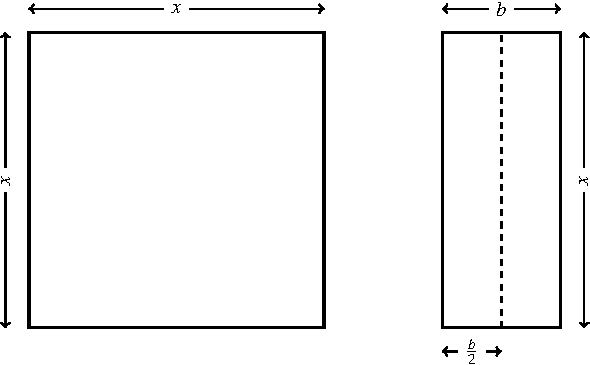
\includegraphics[scale=1.1]{image/10/complete-square-a1-c0.pdf}
\caption{%%
  The quadratic function $f(x) = x^2 + bx$ can be visualised as a
  square plus a rectangle.  The square has a side length of $x$, hence
  the area of the square is $x^2$.  The rectangle has a width of $b$
  and a height of $x$, so the rectangle has an area of $bx$.  Thus
  $f(x)$ can be interpreted as the area of a square plus the area of a
  rectangle.  The rectangle can be cut in half along the dashed line
  as shown.  Each half has a width of $b/2$ and a height of $x$.
}
\label{fig:special_complete_square_square_plus_rectangle}
\end{figure}

\begin{figure}[!htbp]
\centering
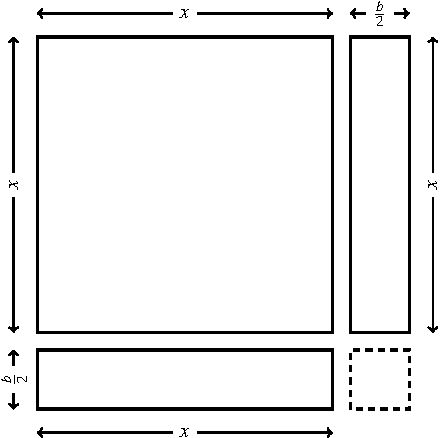
\includegraphics[scale=1.1]{image/10/complete-square-a1-c0_halfb.pdf}
\caption{%%
  The quadratic function $f(x) = x^2 + bx$ can be visualised as a
  square plus a rectangle.  The rectangle is cut in half.  One half is
  arranged to the right of the square.  The other half is arranged
  underneath the square.  Now you have a shape that is nearly like a
  square.  The small dashed square in the lower right is what is
  missing to make a complete square.
}
\label{fig:}
\end{figure}

\end{document}
